Nous allons proposer une définition simple de la convexité pour les \ngones, et plus généralement pour les \ncycles. Ceci demande de savoir que, dans un plan orienté, le triangle non dégénéré $ABC$ est dit \focus{orienté positivement} si la condition $\det \big( \vect{AB} , \vect{AC} \big) > 0$ est validée.
Dans ce cas, le triangle $BAC$ est orienté négativement.


% ----------------------- %


\newpage %TEMPO


\begin{defi} \label{conv-ncycle-def}
	Un \ncycle\ $\setproba{L} = A_1 A_2 \cdots A_n$ est dit \focus{convexe} si  l'une des alternatives suivantes a lieu.
    %
	\begin{itemize}
		\item $\forall (i, k) \in \ZintervalC{1}{n}^2$,
		$\det \big( \vect{\primeit{A}_i \primeit{A}_{i+1}}, \vect{\primeit{A}_i \primeit{A}_k} \big) \geq 0$.

		\item $\forall (i, k) \in \ZintervalC{1}{n}^2$,
		$\det \big( \vect{\primeit{A}_i \primeit{A}_{i+1}}, \vect{\primeit{A}_i \primeit{A}_k} \big) \leq 0$.
    \end{itemize}
	
	Autrement dit, $\setproba{L} = A_1 A_2 \cdots A_n$ est convexe si l'une des alternatives suivantes a lieu.
    %
	\begin{itemize}
		\item $\forall (i, k) \in \ZintervalC{1}{n}^2$,
		$\primeit{A}_i \primeit{A}_{i+1} \primeit{A}_k$ est soit dégénéré, soit  orienté positivement.

		\item $\forall (i, k) \in \ZintervalC{1}{n}^2$,
		$\primeit{A}_i \primeit{A}_{i+1} \primeit{A}_k$ est soit dégénéré, soit  orienté négativement.
    \end{itemize}
\end{defi}


\begin{remark}
    Voici des exemples pour clarifier le vocabulaire.	
    
    \begin{center}
    	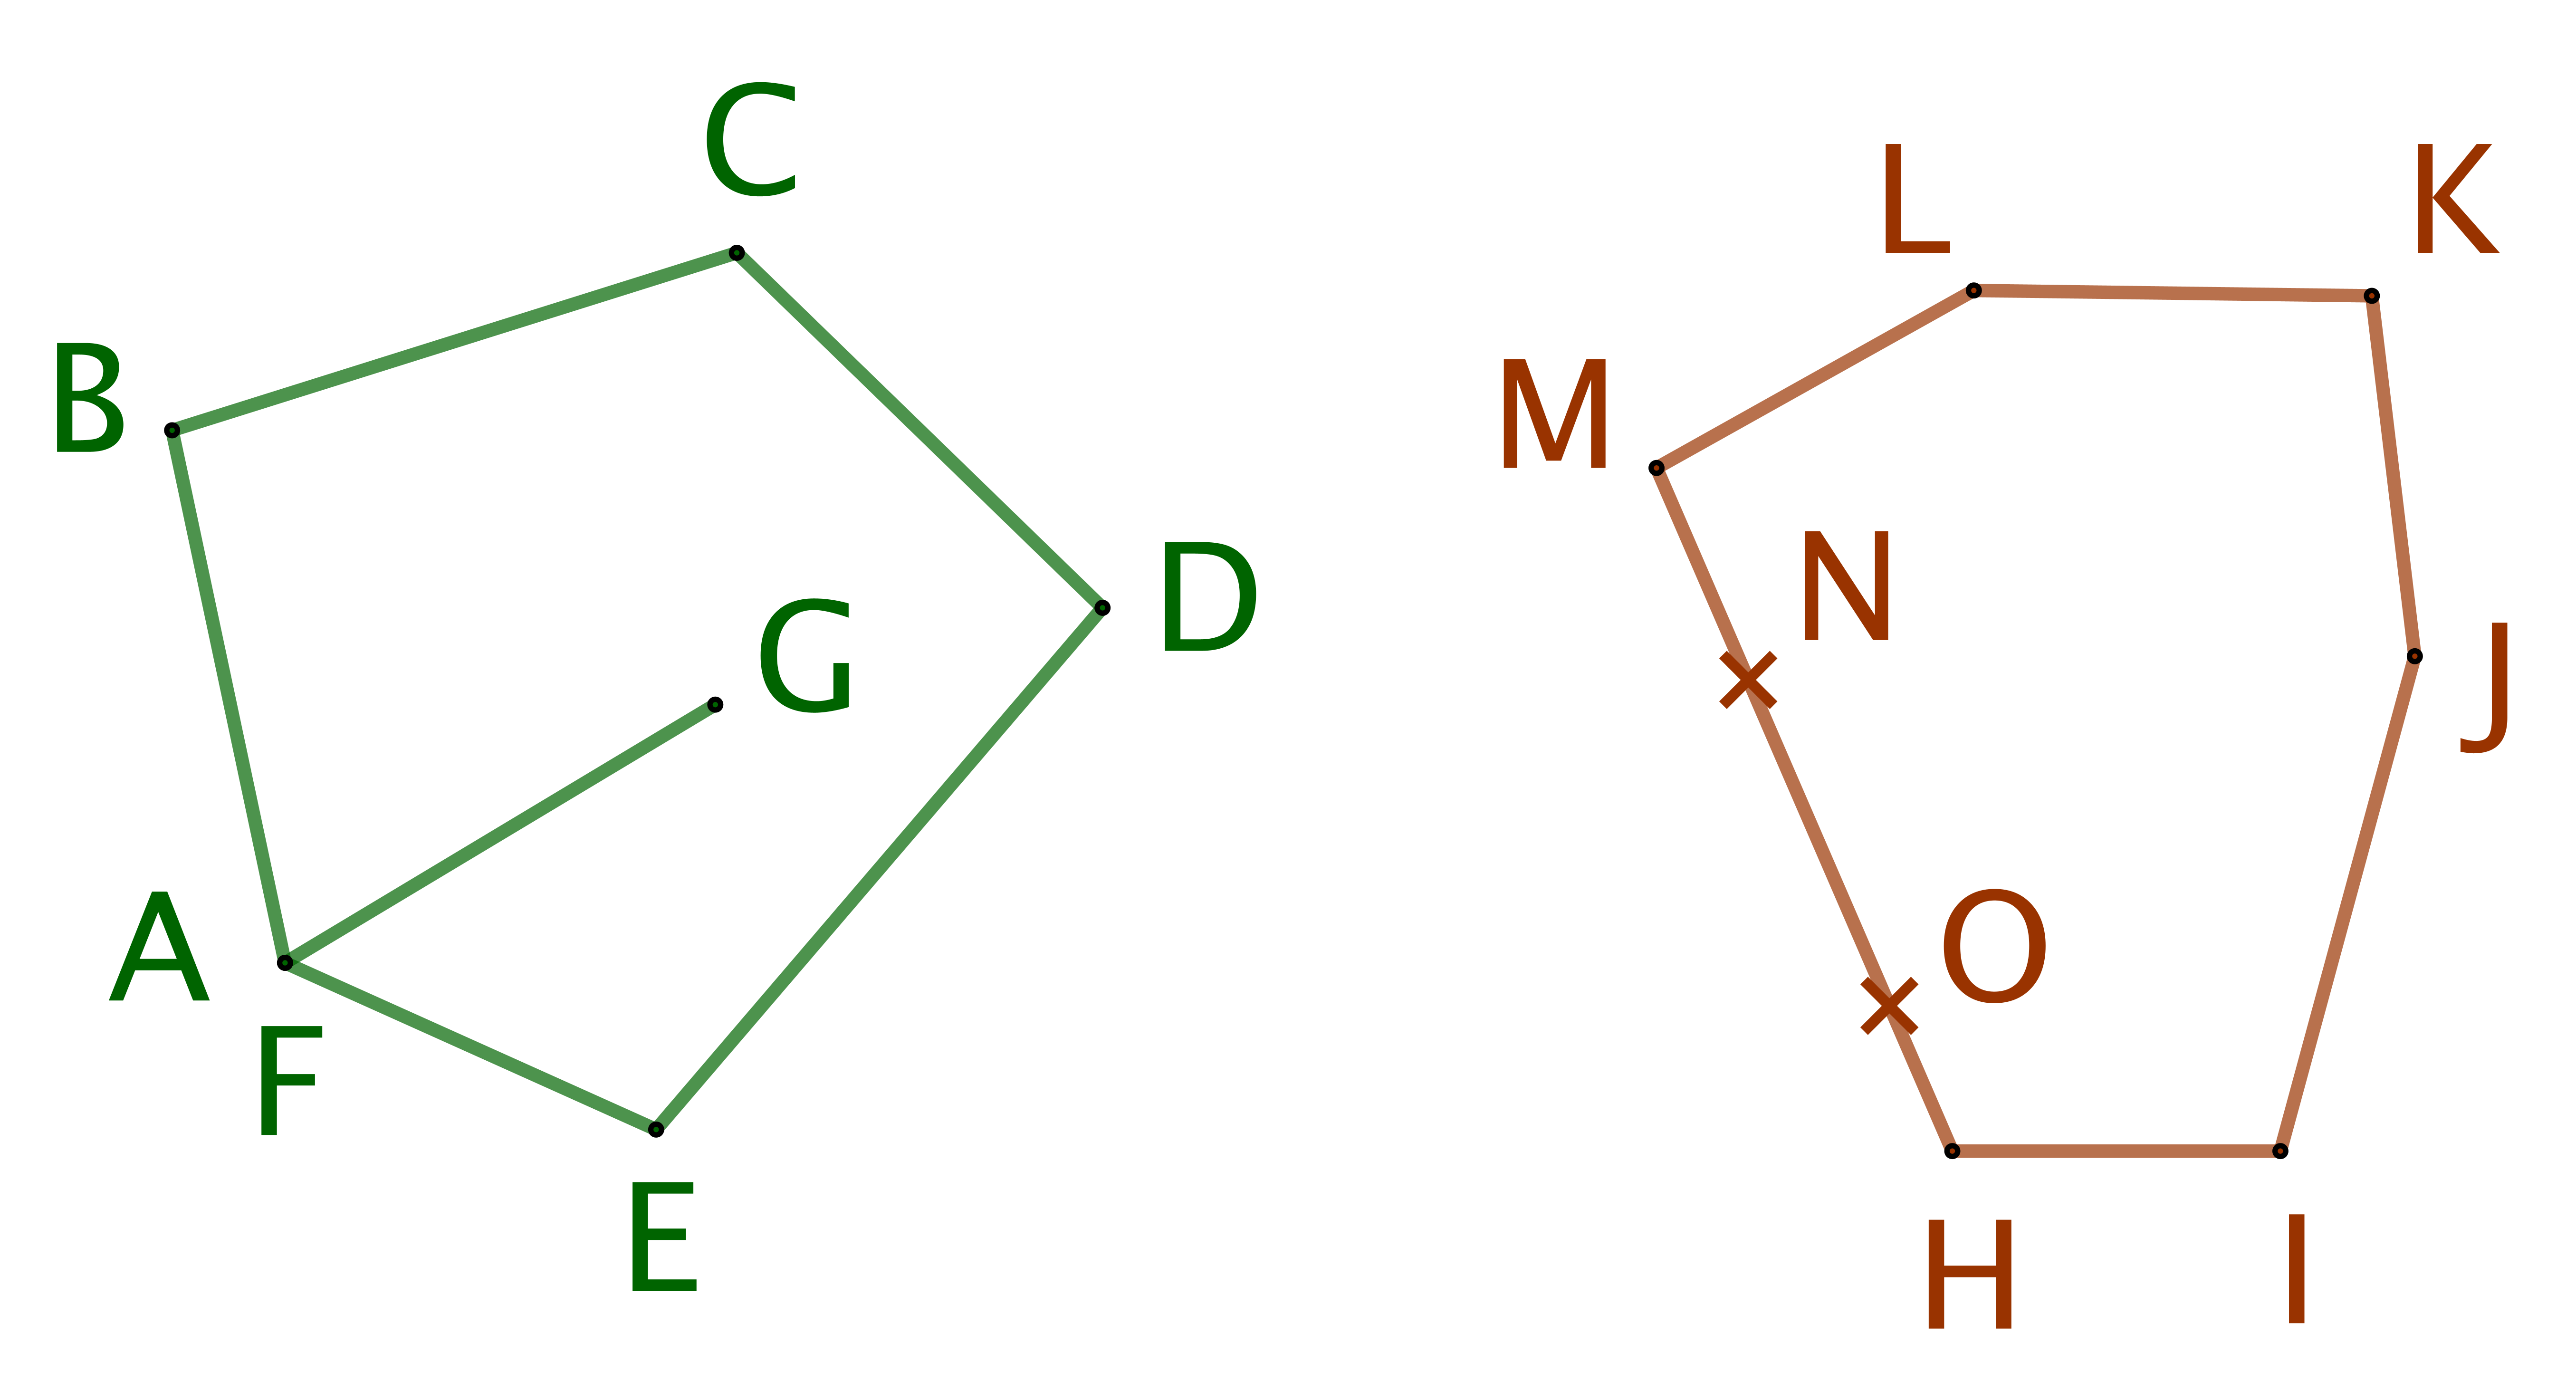
\includegraphics[scale=.3]{content/polygon/convex/degenerated-ncycles.png}
    \end{center}
    
    Le \xcycle{7} non dégénéré $ABCDEFG$ n'est pas convexe, à cause, par exemple, des triangles d'orientations opposées $FGE$ et $FGC$.%
    \footnote{
        $ABCDEFG$ n'est pas un \xgone{7}, car les trois sommets consécutifs $F$, $G$ et $A$ sont alignés.
    }
    Par contre,
    le \xcycle{8} dégénéré $HIJKLMNO$ est convexe, contrairement à $HIJKLMON$, à cause, par exemple, de $MOK$ et $ONK$.%
    \footnote{
         Cet exemple montre que la caractérisation classique de la convexité d'un polygone en terme de demi-espace fermé n'est pas assez précise pour les \ncycles. Ceci est normal, à cause de la possibilité de dégénérescence.
    }
    Enfin,
    $HIJKLM$ est un hexagone convexe.
\end{remark}


% ----------------------- %







\newpage

.%
\footnote{
    Pourquoi s'attarder sur des inégalités larges? Parce que nous allons travailler dans un ensemble compact, et donc fermé, de \ncycles.
    Pour garder des \ngones, nous devrions utiliser des non-égalités, mais ceci nous ferait sortir du cadre fermé qui nous intéresse.
    Nous n'avons pas le choix!
}

Le fait suivant montre que pour les \ngones\ nous retombons bien sur la définition \focus{classique} de la convexité.%
\footnote{
     Il n'est pas dur de vérifier que le fait \ref{conv-pos-det} implique que tout \ngone\ convexe $\setproba{C}$ vérifie la propriété suivante:
     pour toute paire de points $M$ et $N$ de la surface fermée \focus{intérieure} délimitée par $\setproba{C}$, le segment $[MN]$ est contenu dans cette surface.
}


\begin{fact} \label{conv-pos-det}
    Pour tout \ngone\ convexe $\setproba{P} = A_1 A_2 \cdots A_n$, l'une des alternatives suivantes a lieu (avec des inégalités strictes).
    %
	\begin{itemize}
		\item $\forall (i, k) \in \ZintervalC{1}{n}^2$,
		si $k \notin \setgene{i ; i+1}$, alors
		$\det \big( \vect{\primeit{A}_i \primeit{A}_{i+1}}, \vect{\primeit{A}_i \primeit{A}_k} \big) > 0$.

		\item $\forall (i, k) \in \ZintervalC{1}{n}^2$,
		si $k \notin \setgene{i ; i+1}$, alors
		$\det \big( \vect{\primeit{A}_i \primeit{A}_{i+1}}, \vect{\primeit{A}_i \primeit{A}_k} \big) < 0$.
    \end{itemize}
\end{fact}


\begin{proof}
	Le cas des \xgones{3}, c'est-à-dire des triangles non dégénérés, est immédiat.
	Considérons donc $\setproba{P}$ un \ngone\ convexe pour $n \geq 4$.
	Nous savons que, relativement à $\setproba{P}$, aucun triplet de sommets consécutifs alignés n'existe.
	Dès lors, dans le plan orienté, les trois premiers sommets sont placés suivant l'une des deux configurations suivantes. 
    
    \begin{multicols}{2}
        \small\itshape\centering
       	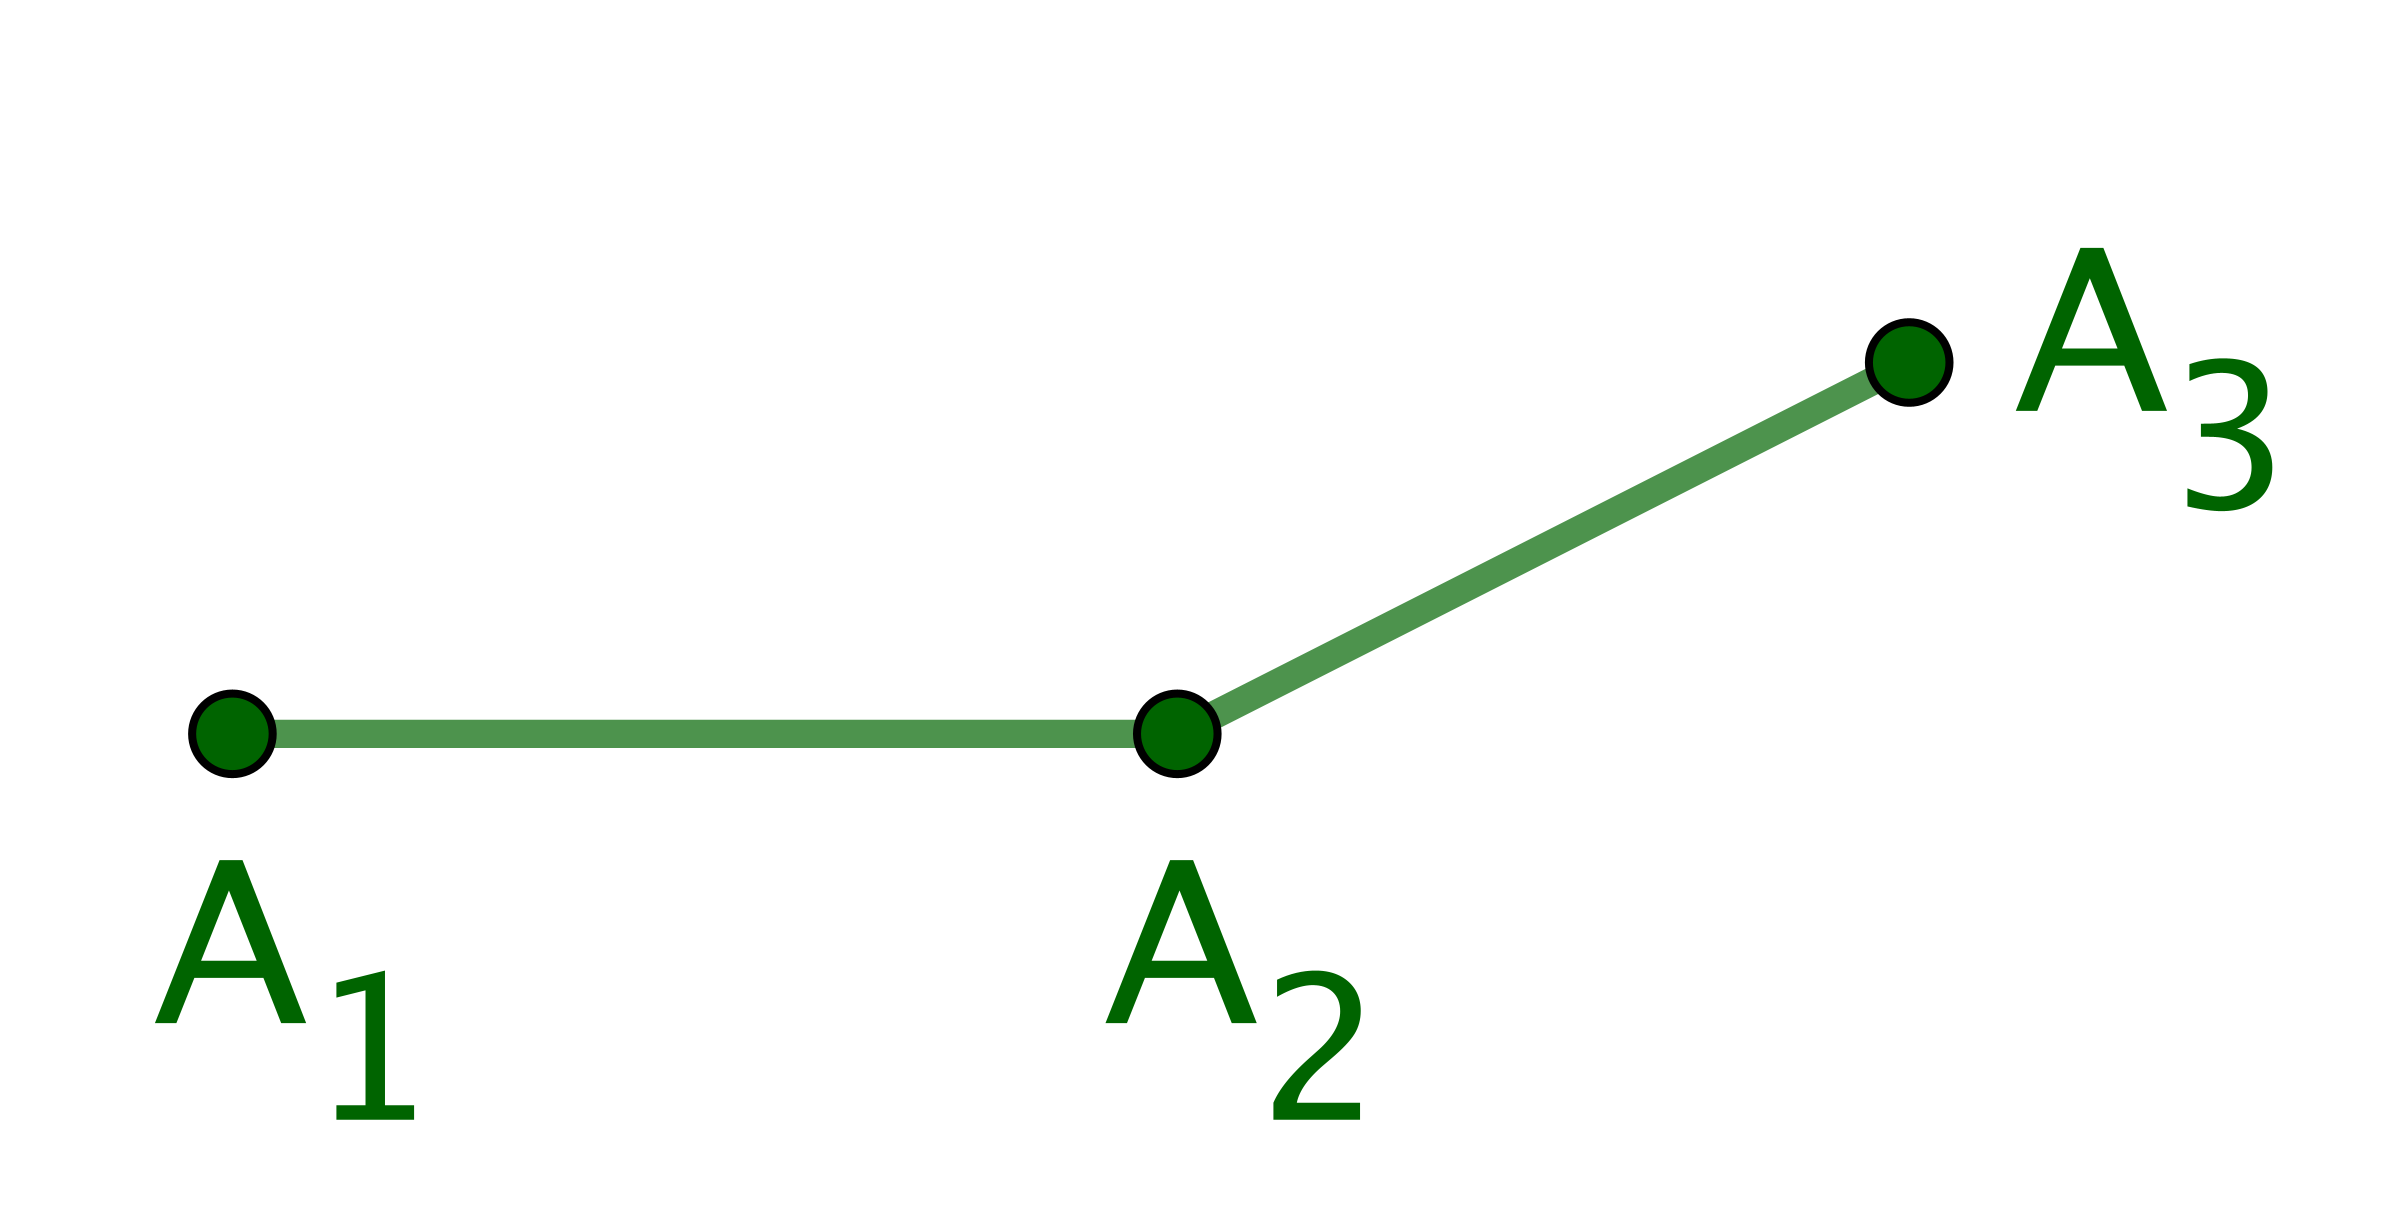
\includegraphics[scale=.45]{content/polygon/convex/conv-det-sign-1.png}
    	    
    	\smallskip
        Cas positif.
        
        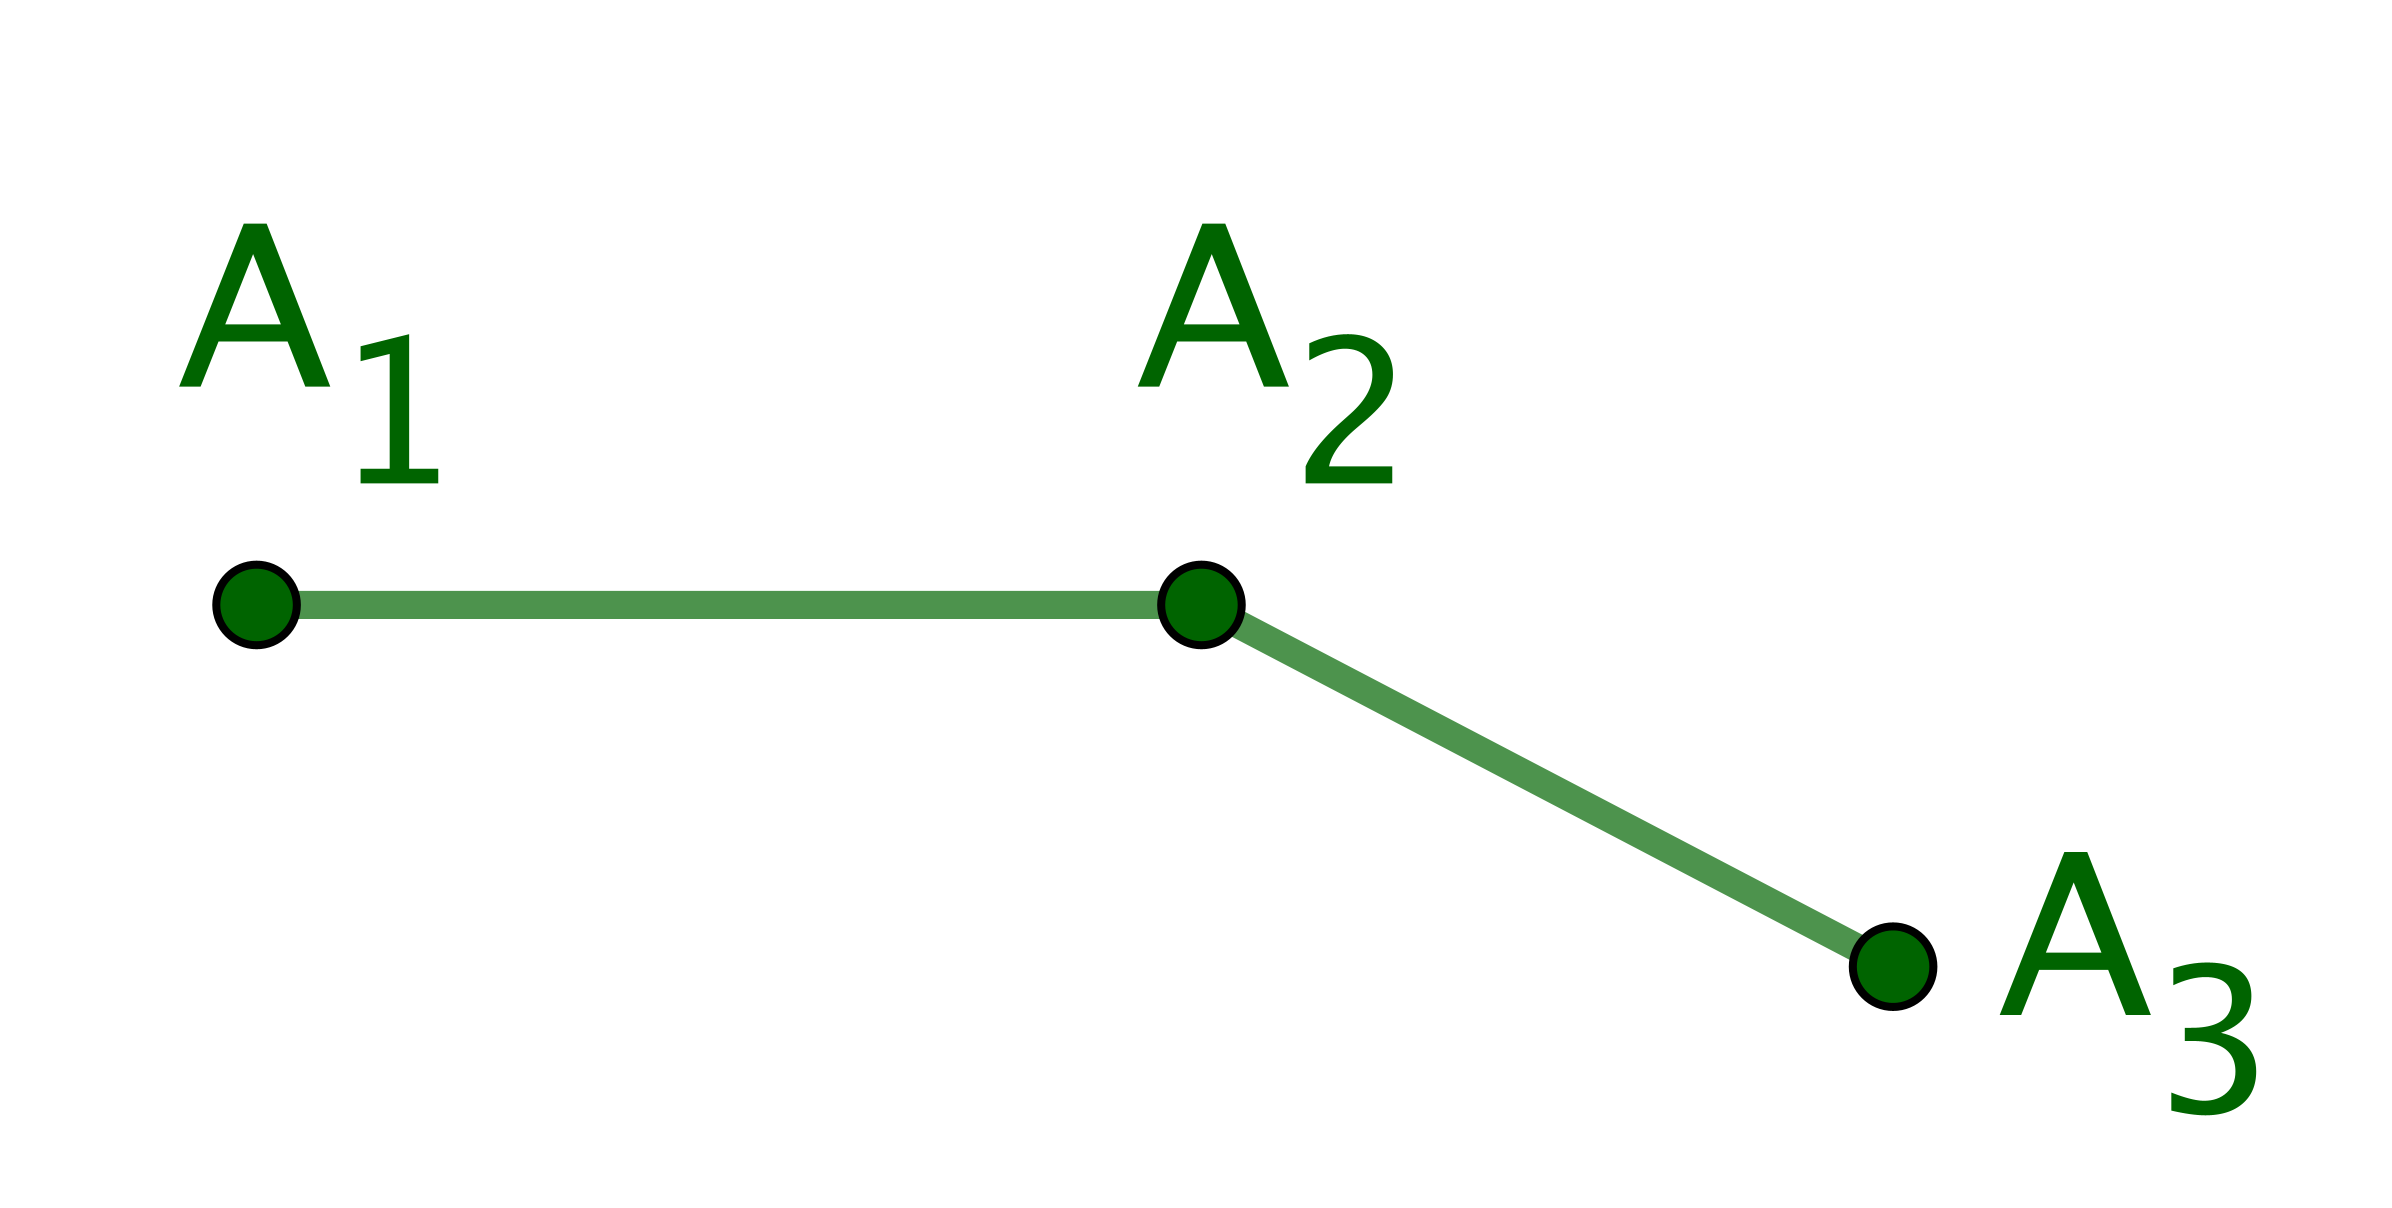
\includegraphics[scale=.45]{content/polygon/convex/conv-det-sign-2.png}
    	    
    	\smallskip
        Cas négatif.
    \end{multicols}

    
%    \newpage


    \noindent
    Considérons le cas positif, c'est-à-dire supposons que 
    $\det \big( \vect{\primeit{A}_1 \primeit{A}_2}, \vect{\primeit{A}_1 \primeit{A}_3} \big) > 0$.
	%
	\begin{itemize}
    	\item $\vect{\primeit{A}_1 \primeit{A}_3} = \vect{\primeit{A}_1 \primeit{A}_2} + \vect{\primeit{A}_2 \primeit{A}_3}$
    	donne
		$\det \big( \vect{\primeit{A}_2 \primeit{A}_3}, \vect{\primeit{A}_2 \primeit{A}_1} \big) > 0$.


		\item Comme $A_2$, $A_3$ et $A_4$ ne sont pas alignés, et de plus $A_1$ et $A_4$ du même côté de la droite $(A_2 A_3)$, au sens large, nous obtenons
		$\det \big( \vect{\primeit{A}_2 \primeit{A}_3}, \vect{\primeit{A}_2 \primeit{A}_4} \big) > 0$.


		\item En continuant de proche en proche, nous arrivons à
		$\det \big( \vect{\primeit{A}_i \primeit{A}_{i+1}}, \vect{\primeit{A}_i \primeit{A}_{i+2}} \big) > 0$
		pour $i \in \ZintervalC{1}{n}$ quelconque.


		\item Le point précédent et la convexité donnent
		$\det \big( \vect{\primeit{A}_i \primeit{A}_{i+1}}, \vect{\primeit{A}_i \primeit{A}_k} \big) \geq 0$
		pour $(i, k) \in \ZintervalC{1}{n}^2$ tel que $k \notin \setgene{i ; i+1}$.


		\item
		Montrons maintenant que
		$\det \big( \vect{\primeit{A}_1 \primeit{A}_2}, \vect{\primeit{A}_1 \primeit{A}_k} \big) > 0$
		pour $k \in \ZintervalC{3}{n}$.
		%
		Nous savons déjà l'inégalité vraie pour $k = 3$; passons donc à $k = 4$.
		Pour avoir 
		$\det \big( \vect{\primeit{A}_1 \primeit{A}_2}, \vect{\primeit{A}_1 \primeit{A}_4} \big) > 0$, 
		le point précédent donne qu'il faut vérifier que 
		$\det \big( \vect{\primeit{A}_1 \primeit{A}_2}, \vect{\primeit{A}_1 \primeit{A}_4} \big) = 0$
		est impossible.
		Supposons donc l'égalité vraie, ce qui implique d'avoir $n \geq 5$, car dans le cas contraire les sommets consécutifs $A_4$, $A_1$ et $A_2$ seraient alignés.
		Nous aboutissons aux configurations suivantes où les hachures et la droite en trait plein sont des zones interdites pour $A_4$.

        \begin{multicols}{2}
            \small\itshape\centering
           	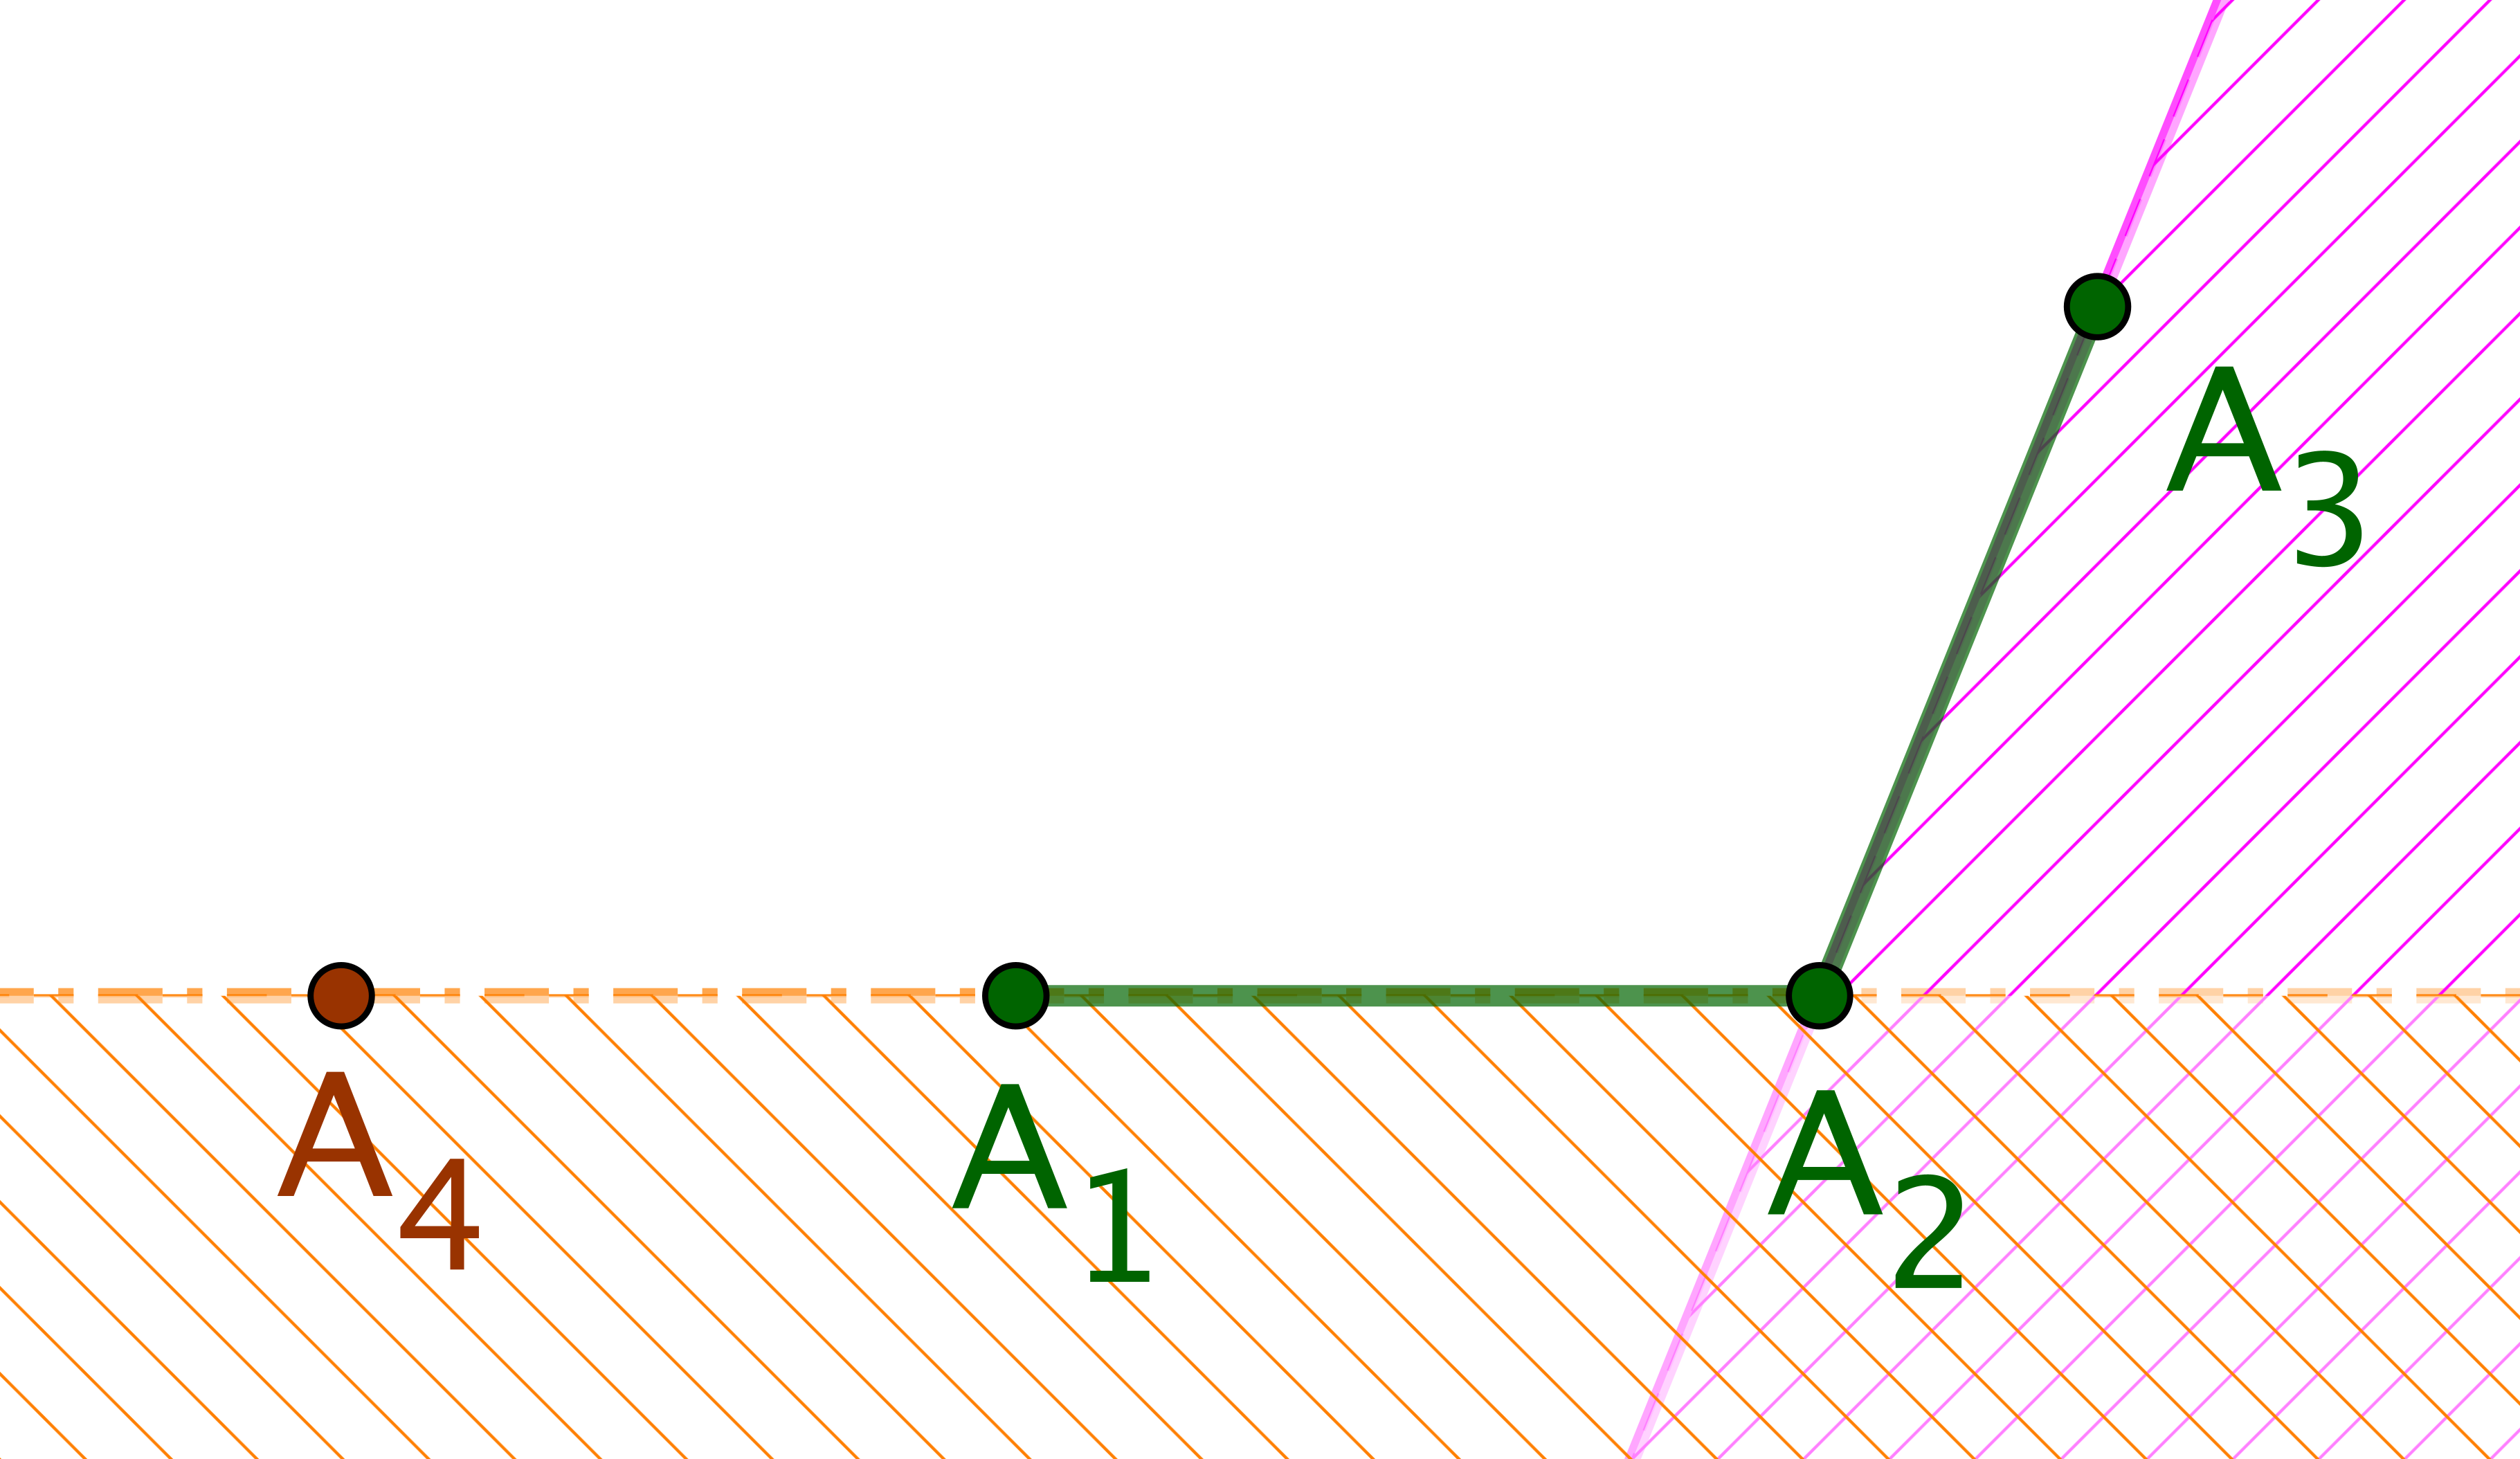
\includegraphics[scale=.4]{content/polygon/convex/conv-det-A4-1.png}
        	    
        	\smallskip
            Cas 1.
            
            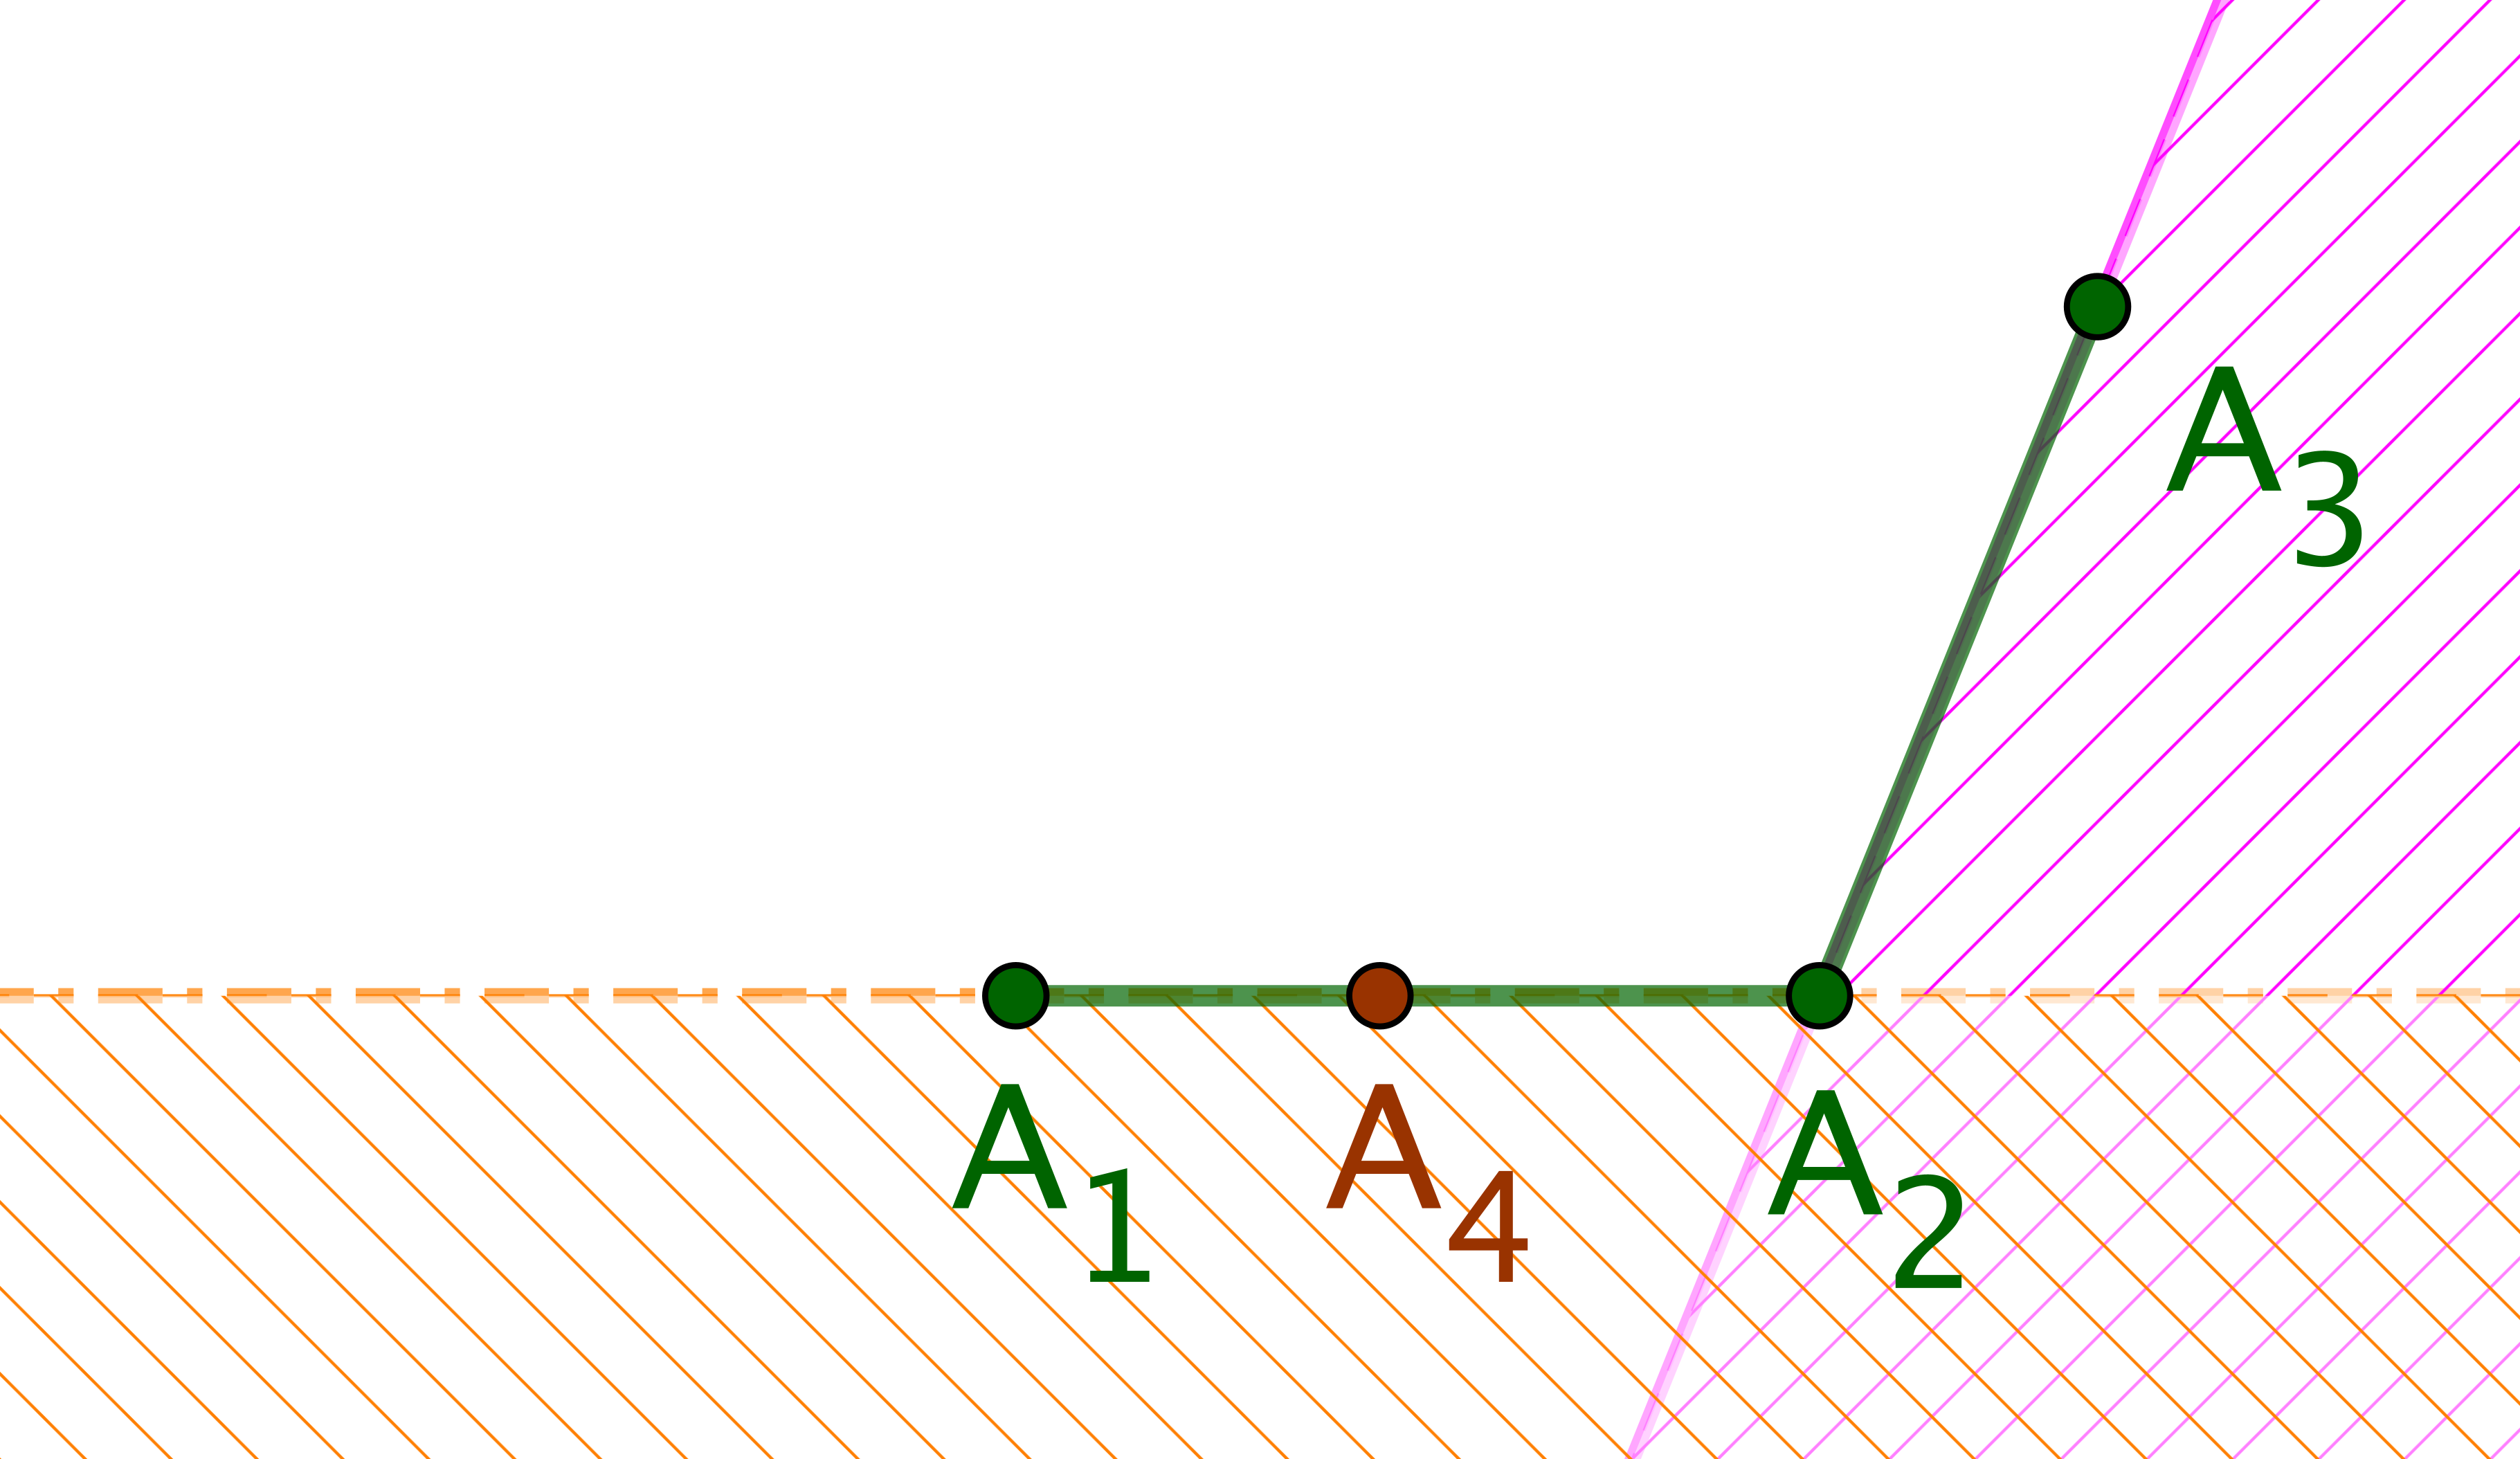
\includegraphics[scale=.4]{content/polygon/convex/conv-det-A4-2.png}
        	    
        	\smallskip
            Cas 2.
        \end{multicols}
    
		\noindent
		Le cas 2 est impossible par raison de convexité, car $A_1$ et $A_2$ sont de part et d'autre de la droite $(A_3 A_4)$. Voyons donc ce qu'implique le 1\ier\ cas pour $A_5$.
		
        \begin{multicols}{2}
            \small\itshape\centering
           	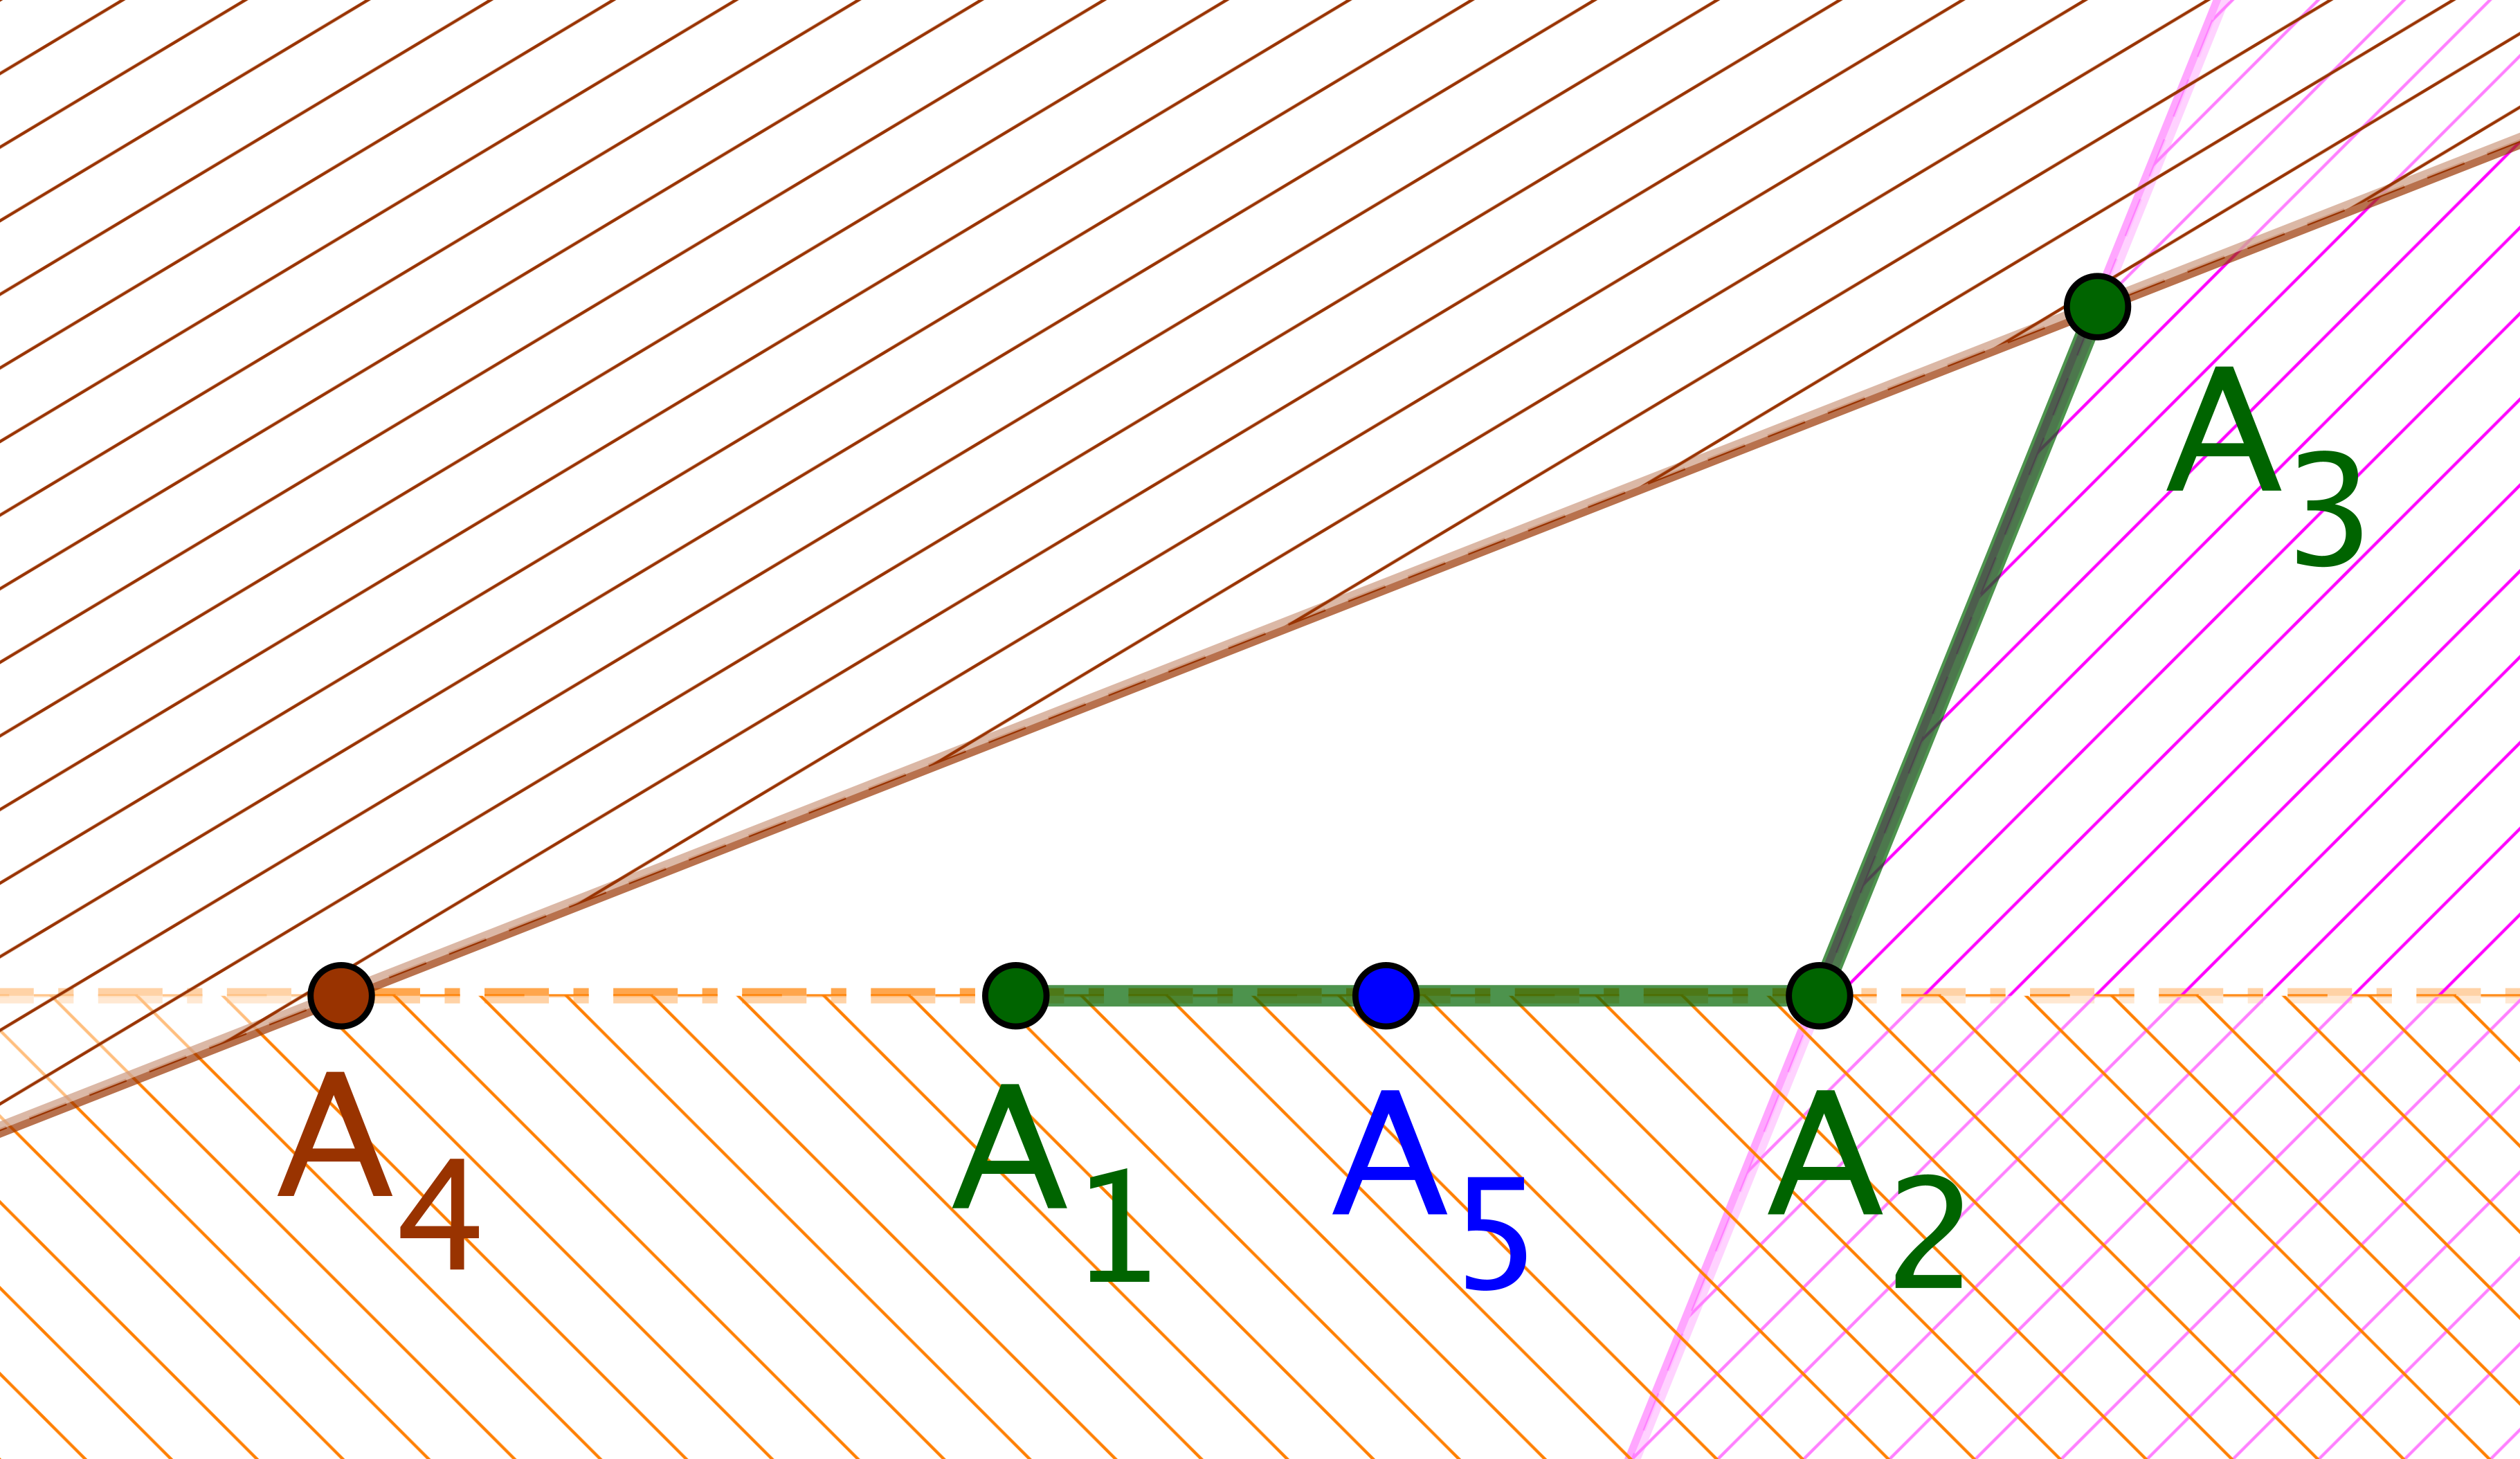
\includegraphics[scale=.4]{content/polygon/convex/conv-det-A5-1.png}
        	    
        	\smallskip
            Cas 1-1.
            
            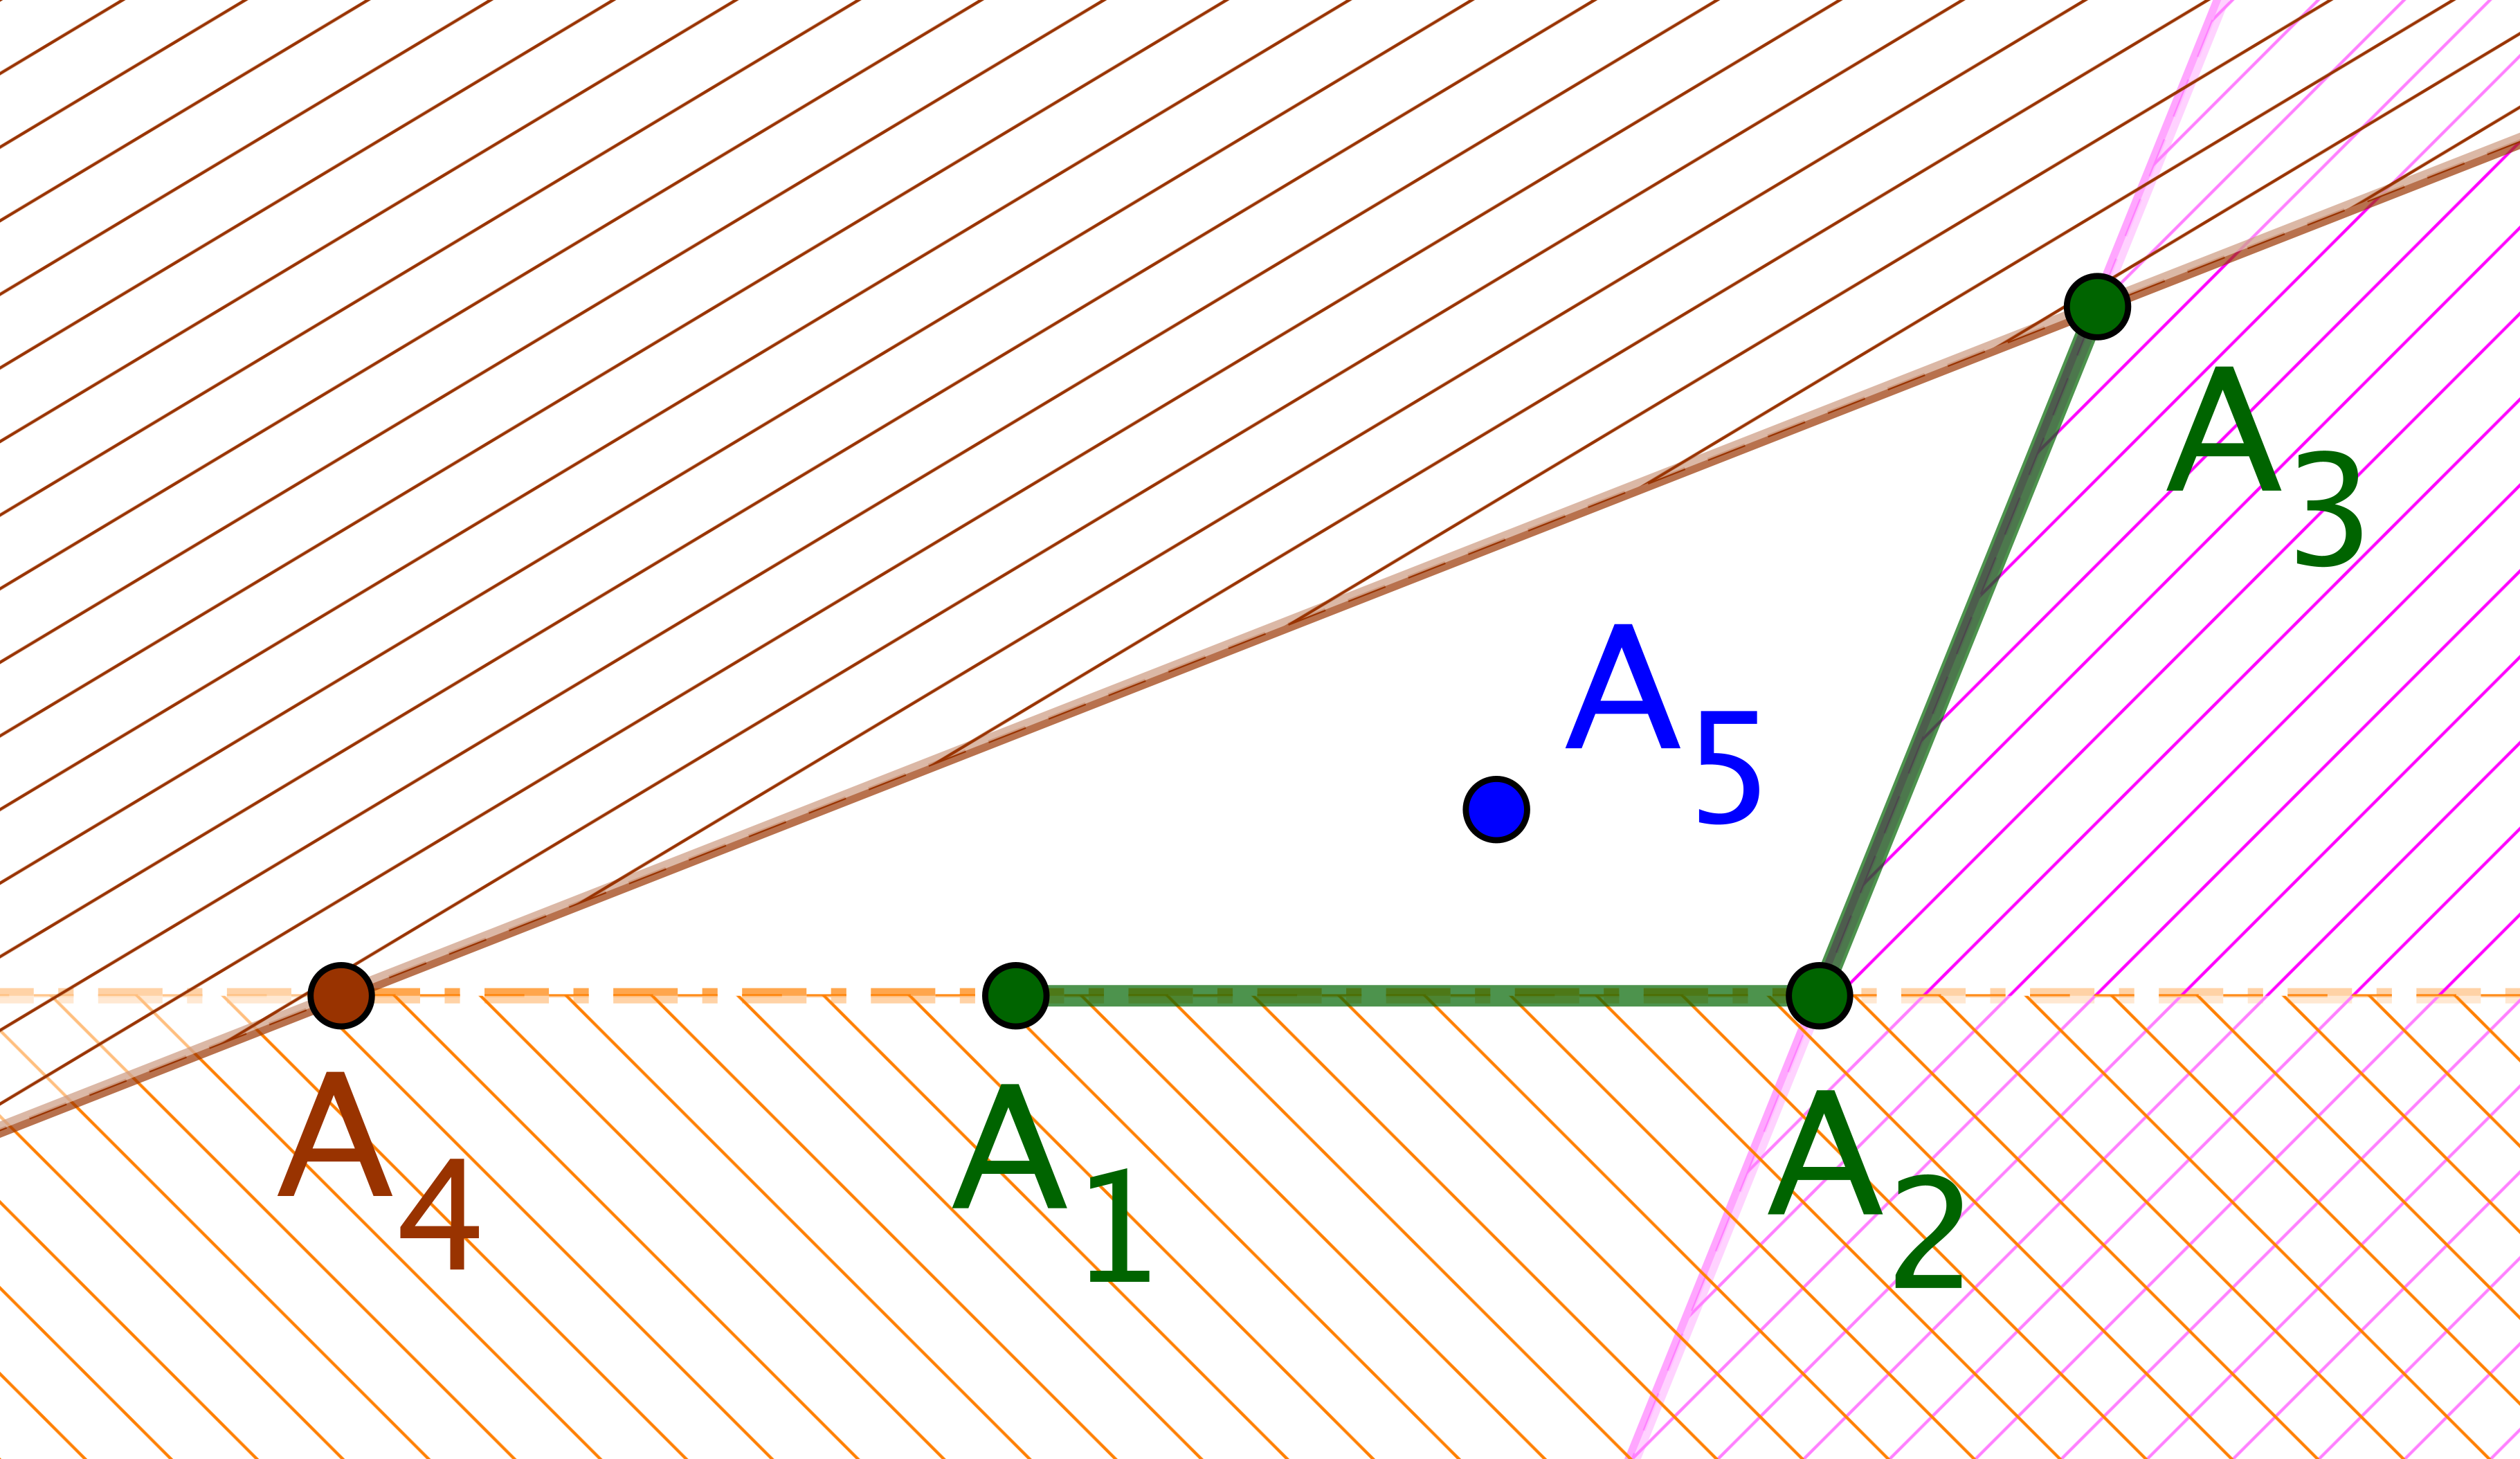
\includegraphics[scale=.4]{content/polygon/convex/conv-det-A5-2.png}
        	    
        	\smallskip
            Cas 1-2.
        \end{multicols}
    
		\noindent
		Le cas 1-2 est impossible par raison de convexité, car $(A_4 A_5)$ sépare les points $A_3$ et $A_2$.
		Notons que dans le cas 1-1, il est possible d'avoir $A_5 \in {]A_4 A_1[}$.
		Comme $A_5 \in (A_1 A_2)$, nous devons avoir $n \geq 6$, 
		mais $A_6$ ne peut être ni à l'intérieur du triangle $A_2 A_3 A_4$ par convexité,
		ni sur la droite $(A_1 A_2)$, car $A_4$, $A_5$ et $A_6$ ne peuvent pas être alignés.
		Cette situation contradictoire montre que
		$\det \big( \vect{\primeit{A}_1 \primeit{A}_2}, \vect{\primeit{A}_1 \primeit{A}_4} \big) > 0$.
		En continuant de même, de proche en proche, nous arrivons à
		$\det \big( \vect{\primeit{A}_1 \primeit{A}_2}, \vect{\primeit{A}_1 \primeit{A}_k} \big) > 0$
		pour $k \in \ZintervalC{3}{n}$.


		\item En généralisant le raisonnement précédent,%
		\footnote{
		    Se souvenir de la définition \focus{cyclique} de la suite $(\primeit{A}_i)$.
		}
		nous avons
		$\det \big( \vect{\primeit{A}_i \primeit{A}_{i+1}}, \vect{\primeit{A}_i \primeit{A}_k} \big) > 0$
		pour tout couple $(i, k) \in \ZintervalC{1}{n}^2$ vérifiant $k \notin \setgene{i ; i+1}$.
	\end{itemize}

    \medskip
    
    \noindent
    Le cas négatif se traite de façon similaire.
\end{proof}


